 \begin{figure*}[thb!]
 	\caption{Approach overview}
 	\centering
 	\label{fig:approach_overview}
 	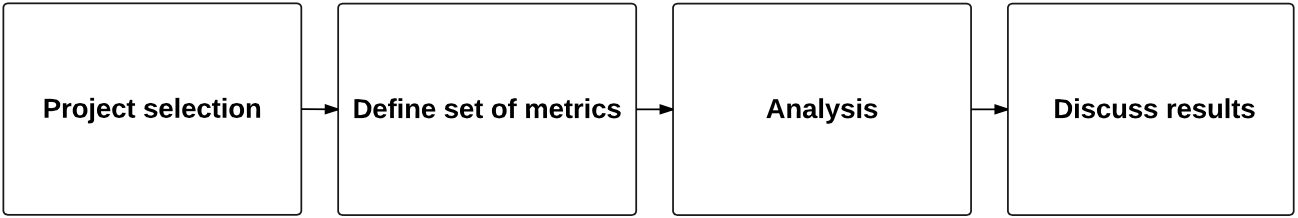
\includegraphics[width=1\textwidth]{figures/approach_overview}
 \end{figure*}
After selecting projects we have to find an automatic way to have all versions downloaded, and ready for analysis. Instead of downloading each version separately, we devise a viable and more efficient technique. We cloned latest release containing \textit{\.git} folder in it. Then we write a script to checkout each tag based on the tags that git gives us by running \textit{git tag}.
\par
Each version of each application has been analyzed with a powerful source code analyzer tool named SonarQube to extract metrics relevant to evolution of software. We also used this tool catch anti-patterns developers do in JavaScript and categorize them based on their severity.
To have all these data get analyzed in SonarQube we had to deal few unexpected behavior. For example SonarQube does not consider release dates as the real release date. It just take out the date of the analysis that it fires to analyze a source. In this scenario we have 1065 releases with the release date of the day we ran analysis. So we fixed the issue to have proper release dates.



\par After analyzing every tag in SonarQube we extract our chosen metrics that we found them proper for studying evolution of JavaScript projects. Metrics such as McCabe cyclomatic complexity,  comment line density, duplicated lines and blocks, number of directories and statements and etc. Table  \ref{tab:metrics_definition} defines sets of metrics that we used in our analysis.



\par
Lehman suggests using the number of “modules” as the best way to measure the size of a large software system \cite{Lehman1997METRICS}. However, we decided to use the number of uncommented lines of code (“uncommented LOC”) like the way Godfrey et al \cite{Godfrey2000ICMS} did the evolution study on Linux Kernel. On the other hand we measure the comment lines and the ratio of comments to lines of codes, and based on that we can infer how much developers tend to put comments within their codes. We have to consider hidden corners that can mislead results, for example descriptive comments are totally different to the lines of codes that got commented because of refactoring or changes which consider as light-weight code smells within the code.

We want to measure various aspects of the growth of these applications by having metrics such as number of files, lines of code, number of functions and statements. We also measure amount of duplications known as clones in terms of lines of codes, blocks and files. We would measure the cyclomatic complexity over time which the metric is calculated as following. Whenever the control flow of a function splits, the complexity counter gets incremented by one. Each function has a minimum complexity of 1. The control flow can split by conditional statements like if/else, switch case and so on. This metric is also known as also known as McCabe metric
We use the term “source file” to mean any file whose name ends with \textit{“.js”} and also we removed folders containing external libraries which is usually located at \textit{lib} or \textit{node\_modules}. 


\begin{table*}[!hbt]
	\begin{center}
		\caption{Selected metrics definition}
		\label{tab:metrics_definition}
		\begin{tabular}{c| l l }
			\toprule
			
			\textbf{Metric} & \textbf{Definition} \\ \midrule
			Lines of Code & The number of uncommented lines of code    \\
			Complexity      & McCabe complexity    \\
			Complexity/function & Average complexity by function. \\
			Complexity/file & Average complexity by file \\
			Comment lines  & Number of lines containing either comment or commented-out code. \\
			Comment Lines (\%)   & Density of comment lines = Comment lines / (Lines of code + Comment lines) * 100    \\
			Duplicated lines (\%)     & Density of duplication = Duplicated lines / Lines * 100    \\
			Duplicated blocks   & Number of duplicated blocks of lines    \\
			Directories   & Number of directories    \\
			Functions            & Number of functions    \\
			Statements      & Number of functions   \\
			Issues    & Number of issues with severity of blocker, critical, major and minor   \\
			Technical debt    & Number of days it takes to fix issues with respect to their severity    \\
			Technical debt ratio   & Division of SQALE Index by the estimation effort to re-develop your application from scratch.    \\
		\end{tabular}
	\end{center}
\end{table*}


